\documentclass[xcolor=dvipsnames]{beamer}
\usepackage{tikz}
\usepackage{url}
\usepackage{tabularx}
\usepackage{multirow}
\usecolortheme[named=Plum]{structure} 
\usetheme[height=7mm]{Rochester} 
\setbeamertemplate{navigation symbols}{} 
\title[Pacemaker introduction]{Introduction  to Pacemaker}
\author{Paulius and Bogdan}
%\date{Jule 13, 2007}

\begin{document}
  \begin{frame}
    \titlepage
  \end{frame}

  \begin{frame}
    \frametitle{Heart}
    \begin{figure}
      \begin{center}
        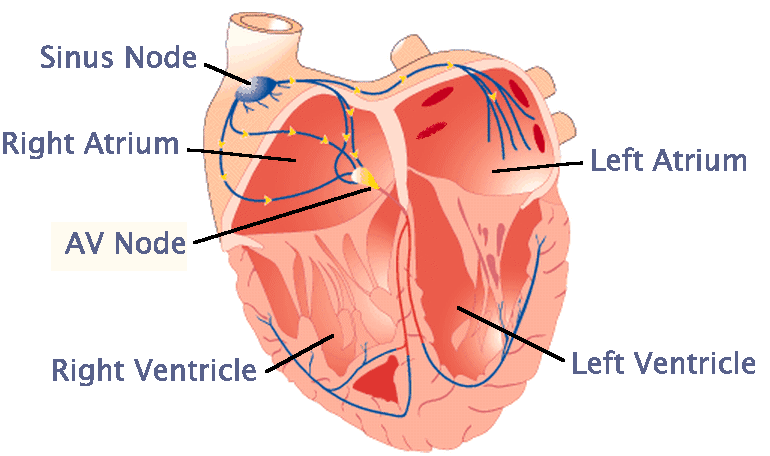
\includegraphics[width=0.7 \textwidth]{Figures/heart.png}
        \footnote{\url{http://www.a-fib.com/images/Steve's\%20Heart\%20Illustration\%20Final\%20Left-Right-Node\%20Corrected.gif}}
      \end{center}
    \end{figure}

    Heart is a pump with four chambers: 
    \begin{itemize}
      \item Atria - top 2 chambers
      \item Verticles - bottom 2 chambers
    \end{itemize}
  \end{frame}

  \begin{frame}
    \frametitle{Heartbeat}
    Cardiac cycle is a sequence of events that happens during single heartbeat. During cardiac cycle blood enters atria and is pumped out of the verticles.

    A normal resting heart rate range is 60 - 100 beats per minute (bpm). During extreme exercise it can reach 220 bpm.

    \begin{enumerate}
      \item SA (Sinoatrial) node sends impuls to AV node through atria
      \item Atria chambers contracts
      \item AV (Atrioventricular) node sends impuls to ventricles
      \item Ventricles contract 
    \end{enumerate}
  \end{frame}

  \begin{frame}
    \frametitle{Electrocardiography (ECG or EKG)}
    \begin{columns}
      \begin{column}{0.5\textwidth}
        ECG represents electrical changes during cardiac cycles over time.

        ECG of a single cardiac cycle is shown on the right.

        \begin{itemize}
          \item P wave denotes current that causes atrial contraction.
          \item QRS is current that invokes contraction in verticles.
          \item T wave represents repolarization of the ventricles. Atrial repolarization is obscured by QRS.
        \end{itemize}

      \end{column}
      \begin{column}{0.5\textwidth}

        \begin{figure}
          \begin{center}
            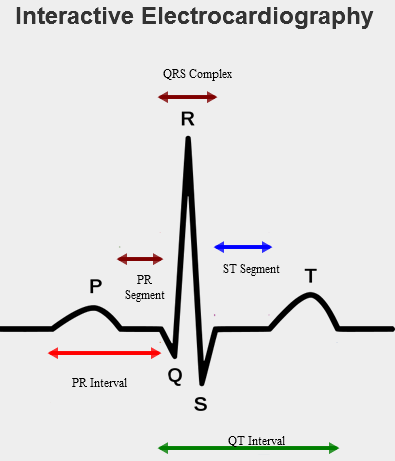
\includegraphics[height=0.7 \textheight]{Figures/ecg.png}
            \footnote[frame]{\url{http://www.imapbuilder.com/customization/images/interactive\_electrocardiography.png}}
          \end{center}
        \end{figure}
      \end{column}
    \end{columns}
  \end{frame}

  \begin{frame}
    \frametitle{Intervals in cardiac cycle}
    If person has 60 bbm, then cardiac cycle is 1 second long.
    \begin{itemize}
      \item P wave - 0.06 to 0.12 seconds
      \item PR interval - 0.12 to 0.20 sec
      \item QRS complex - 0.06 to 0.10 sec
      \item ST segment - 0.08 to 0.12 sec
      \item T wave - 0.10 to 0.25 sec
      \item QT interval - depends on heart rate
      \item U wave recovery of Purkinje fibers in ventricles - usually not present in ECG.
    \end{itemize}


  \end{frame}

  \begin{frame}
    \frametitle{Pacemaker}
    Has two main functions:
    \begin{itemize}
      \item Sensing 
      \item Pacing of the heart
    \end{itemize}

    Pacemaker can only accelerate the heart. It never slows it down. 

    Typically pacemakers have components to detect physical activity (rate sensing). 

    Pacemaker sends impuls through the lead connected to the heart:
    \begin{itemize}
      \item Single-chamber pacemaker has one lead. 
      \item Double-chamber pacemakar has two leads.
    \end{itemize}
  \end{frame}

  \begin{frame}
    \frametitle{Pacemaker}
    \begin{figure}
      \begin{center}
        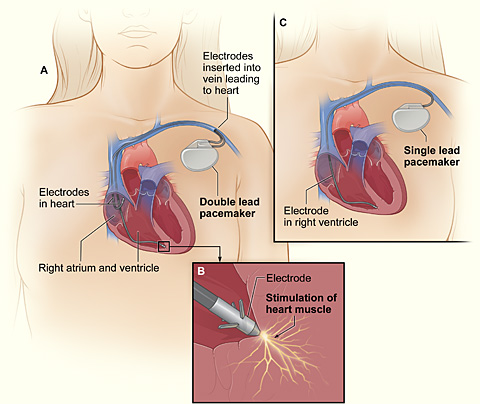
\includegraphics[width=1 \textwidth]{Figures/pacemaker.png}
      \end{center}
    \end{figure}
  \end{frame}

  \begin{frame}{}
    \frametitle{Pacemaker modes}
    Different heart abnormalities require different pacing modes. Pacing modes are described using classification code. Code can have between 3 to 5 positions.

    \begin{tabularx}{\textwidth}{|X|X|X|X|}
      \hline
              Chamber(s) Paced & Chamber(s) Sensed & Response To Sensing & Rate Modulation  \\ \hline
              0-None           & 0-None            & 0-None              & \multirow{2}{2cm}{R-Rate Modulation}  \\ % \hline
              A-Atrium         & A-Atrium          & T-Triggered         &                    \\ % \hline
              V-Ventricle      & V-Ventricle       & I-Inhibited         &                    \\ % \hline
              D-Dual           & D-Dual            & D-Tracked           &                  \\
      \hline
    \end{tabularx}

  \end{frame}

  \begin{frame}
    \frametitle{First position}
Describes the heart chamber that is paced.
\begin{itemize}
  \item O - No pacing
      \item A - Pacing occurs in the atria only
      \item V - Pacing occurs in the verticles only
      \item D - Pacing occurs in both atra and verticles
\end{itemize}
  \end{frame}

  \begin{frame}
    \frametitle{Second position}
Describes the heart chamber that is sensed.
\begin{itemize}
  \item 0 - No sensing
  \item A - Sensing occurs in the atria only
  \item V - Sensing occurs in the verticles only
  \item D - Sensing occurs in both atra and verticles
\end{itemize}

  \end{frame}

  \begin{frame}
    \frametitle{Third position}
    Describes what pacemaker does if it senses intrinsic heart electrical activity in the monitored chambers
  \begin{itemize}
    \item 0 - Emits a pulse to selected chamber at a set interval (fixed rate)
    \item T - Emits a pulse only if sensed event occured
    \item I - If intrinsic activity is faster than a set rate (sensed event occurs), it inhibits pacing. Otherwise, it pacing starts.
    \item D - Will inhibit a pulse if intrinsic event sensed. Will emit pulse in the ventricle if it sensed intrinsic event in atrium, but did not sense a pulse in the ventricle (Requires dual chamber pacemaker)
  \end{itemize}

  \end{frame}

  \begin{frame}
    \frametitle{Fourth position and DDD explanation}
    Rate responsive pacemakers can sense patients activity level and adapt to changes.\par
    
    \hrulefill\par 
    In DDD mode, pacemaker:
    \begin{enumerate}
      \item Senses atrium and ventrical intrinsic activity
      \item If after certain interval no intrinsic atrium pulse sensed, pacemaker emits atrium pulse; otherwise inhibit pulse
      \item If after certain interval no intrinsic ventricle pulse, pacemaker emits ventrical pulse; otherwise inhibit pulse
    \end{enumerate}

  \end{frame}

  \begin{frame}
    \frametitle{Pacemaker cardiac cycle}
    \begin{itemize}
      \item Pacemaker uses programmable sensitivity parameters to detect P, R and T waves. Measured in millivolts.
      \item P and T waves have similar voltages.
      \item T wave detection: pacemaker paces or senses ventricular event and waits ventricular refractory period.
    \end{itemize}
  \end{frame}
  
  \begin{frame}
    \frametitle{Configuration parameters}

  \end{frame}



\end{document}

